\PassOptionsToPackage{hyphens}{url}
\documentclass[11pt,a4paper]{article}
\usepackage[T1]{fontenc}
\usepackage[utf8]{inputenc}
\usepackage[spanish,es-noquoting,es-tabla]{babel}
\usepackage{amsmath,amssymb}
\usepackage{booktabs}
\usepackage{graphicx}
\usepackage[margin=2.2cm]{geometry}
\usepackage{microtype}
\usepackage[colorlinks=true,linkcolor=black,urlcolor=blue,citecolor=black]{hyperref}
\usepackage{xcolor}
\usepackage{enumitem}
\usepackage{listings}
\usepackage[most]{tcolorbox}
\urlstyle{tt}
\setlist{nosep,leftmargin=1.4em}

% código: las líneas importantes van entre @| |@ y salen en rojo oscuro, negrita
\lstdefinestyle{f90}{language=[90]Fortran,basicstyle=\ttfamily\scriptsize,
  columns=fullflexible,keepspaces=true,keywordstyle=\color{blue!45!black},
  commentstyle=\color{gray}\itshape,numbers=left,numberstyle=\tiny\color{gray},
  numbersep=5pt,frame=single,framerule=0.3pt,rulecolor=\color{gray!70},
  xleftmargin=2.2em,xrightmargin=0.5em,aboveskip=3pt,belowskip=3pt,
  moredelim=**[is][\color{red!65!black}\bfseries]{@|}{|@}}

\newcommand{\etq}[1]{\textcolor{gray}{\texttt{[#1]}}}
\newcommand{\archivo}[1]{\nolinkurl{#1}}
\makeatletter\g@addto@macro{\UrlBreaks}{\do\_\do\-\do\.}\makeatother
\newcommand{\propio}{\textsuperscript{\textcolor{gray}{\,\S}}}
\newcommand{\Tr}{\mathrm{Tr}}
\graphicspath{{../salidas/figuras/}}

% resultados de numerico/fase6/escaleras.py (se completan desde los JSON)
\newcommand{\NLunoOrd}{1,00 y 1,00}
\newcommand{\NLtresOrd}{2,33 y 3,02}
\newcommand{\NLtresErr}{órdenes 2,33 y 3,02, con errores de $6{,}9\cdot10^{-7}$ a $2{,}8\cdot10^{-5}$ para $\varepsilon=0{,}01$ a $0{,}04$, contra $5\cdot10^{-3}$ a $2\cdot10^{-2}$ de $N=1$}

\title{\vspace{-1.2cm}Superficie deformable de orden $N$ en SPECTER\\[2pt]
\large resumen para leer --- qué se hizo, qué encontró y dónde está el código}
\author{Lucía Mazaira \quad\small INFINA, CONICET--UBA}
\date{\small 28 de septiembre de 2026}

\begin{document}
\maketitle
\vspace{-0.6cm}

\begin{tcolorbox}[colback=gray!5,colframe=gray!60,boxrule=0.4pt,left=6pt,right=6pt,top=4pt,bottom=4pt,
  title={En una página},fonttitle=\bfseries\small,coltitle=black,colbacktitle=gray!15]
\small
\textbf{Qué se construyó.} Un camino nuevo de SPECTER (\archivo{src/boundary/fsorder.f90}) que
impone en $z=L_z$ las condiciones \emph{exactas} de la superficie $z=h+\eta$, desarrolladas en
Taylor en $\eta$ y truncadas a orden $N=1,2,3$ en la amplitud, con el volumen de Navier--Stokes
completo. Se activa con \texttt{fsorder = 2} o \texttt{3}; $N=1$ reproduce la superficie lineal
de la Fase~5 a $2{,}5\cdot10^{-15}$.

\textbf{Qué funciona.} $N=3$, estable para todo $\eta$ probado ($-4\Delta z$ a $+9\Delta z$)
con $\nu\,dt/\Delta z^2\le0{,}19$. $N=2$, estable para cualquier $\eta>0$, y para $\eta<0$ hasta
$-0{,}667\Delta z$ con el $dt$ de la puerta. La iteración converge en 4--17 pasadas por subpaso. Las funcionales tienen el orden
correcto contra la geometría exacta, y en la onda no lineal $N=3$ tiene orden \NLtresOrd{}
contra 1 de $N=1$.

\textbf{Qué encontró}, las cuatro cosas con evidencia reproducible:
(i)~el cierre que congelé antes de programar es \emph{inestable}, y lo reemplacé;
(ii)~\textbf{el modelo de orden 2 está mal planteado donde $\eta<0$}, ya en el continuo;
(iii)~con elevación media uniforme, $N=2$ ya es $O(\eta^3)$, así que un chequeo de la puerta pedía
el orden equivocado;
(iv)~$\partial_z^3u$ espectral limita a $N=3$ con $n_z=128$.

\textbf{Puerta congelada: 4/10}. Regresiones: Fase~2 6/6 y Fase~5 8/8. Las seis que fallan lo
hacen por límites del modelo o por criterios que fijé mal a priori (§5). Una revisión
independiente en dos rondas, con el rol «verifier», confirmó lo central y encontró nueve cosas.
Ocho las corregí y una queda abierta (§4).

\textbf{Para la celda no aplica nada de esto.} Ahí $\eta/\Delta z\sim10^{-3}$: $1+\sigma\approx1$,
y el error de traza entra multiplicado por $\eta$.
\end{tcolorbox}

\noindent\small Un \propio{} marca derivaciones o estimaciones de esta sesión no validadas contra
bibliografía. El detalle está en \archivo{numerico/fase6/REGISTRO_fase6.md} y en
\etq{D-51}, \etq{D-52}, \etq{H-23}--\etq{H-26}, \etq{V-21}, \etq{V-22} y \etq{P-04} de
\archivo{DECISIONES.md}.\normalsize

%=====================================================================
\section{El modelo}

Con $\Tr_M[f]=\sum_{m=0}^{M}\frac{\eta^m}{m!}\partial_z^m f\big|_{z=L_z}$ ($0$ si $M<0$),
$\mathbf s=\nabla_h\eta$, $S=\nabla\mathbf v+\nabla\mathbf v^{T}$ y $p$ sin la hidrostática del reposo:
\begin{align*}
\partial_t\eta &= \Tr_{N-1}[w]-\mathbf s\cdot\Tr_{N-2}[\mathbf u_h],\\
0 &= \Tr_{N-1}[S_{az}] - s_b\Tr_{N-2}[S_{ab}] + s_a\Tr_{N-2}[S_{zz}] - s_as_b\Tr_{N-3}[S_{zb}],\\
\Tr_{N-1}[p] &= g\eta-\gamma\kappa_N+\nu B_N ,
\end{align*}
con $\kappa_N$ y $B_N$ los truncamientos de la curvatura y de la tensión viscosa normal. Son los
polinomios de Taylor de las condiciones de Wang, Tice \& Kim, ARMA 212 (2014),
\href{https://doi.org/10.1007/s00205-013-0700-2}{10.1007/s00205-013-0700-2}, §1.1,
ecs.~(1.4)--(1.8), leídas en el original. El desarrollo es propio\propio.
\archivo{numerico/fase6/chequeo_expansion.py} lo comprueba con integrales de Cauchy: $10^{-14}$
para $N=1..5$, y $1{,}8$ con el signo de la pendiente cambiado. El verificador lo reprodujo
aparte con series exactas.

«Orden $N$» es en la amplitud, contando la velocidad como de orden de la amplitud: los términos
de velocidad llevan hasta $\eta^{N-1}$. $N=2$ agrega exactamente los términos $\eta\,\partial_z(\cdot)$
y de pendiente que faltaban para el efecto $O(\mathrm{Fr}^2)$ sobre $\alpha$ \etq{H-21}.

%=====================================================================
\section{El código, en tres piezas}

\paragraph{Una pasada de la iteración} (\texttt{fs\_general\_pass}). Las incógnitas de la
superficie son $x=(W,D_x,D_y,P)$:
\begin{itemize}
\item $W=w(L_z)$;
\item $D_{x,y}$, las correcciones de orden $\ge2$ de la tensión tangencial;
\item $P=\sum_{m\ge1}\frac{\eta^m}{m!}\partial_z^m d$, la transferencia de la presión.
\end{itemize}
Las líneas marcadas imponen el dato de Neumann de $\mathbf u^*$ y el Dirichlet del potencial.
Después vienen la proyección y las trazas del estado nuevo; $W$ se resuelve exacto con $B_k$,
como en la Fase~5.
\begin{lstlisting}[style=f90,firstnumber=540]
      ind = planfc%z%n - planfc%z%c
      DO i = ista,iend
         DO j = 1,planfc%y%n
@|            vx(ind,j,i) = im*kx(i)*(wst(j,i) - 2*x(j,i,1)) - x(j,i,2)|@
@|            vy(ind,j,i) = im*ky(j)*(wst(j,i) - 2*x(j,i,1)) - x(j,i,3)|@
@|            dtop(j,i) = dtop0(j,i) - x(j,i,4)|@
         ENDDO
      ENDDO
      CALL neumann_reconstruct(planfc,vx,6,1)
      CALL neumann_reconstruct(planfc,vy,6,1)
      CALL goto_3d_fourier(planbc,planfc,vx,vy)
      CALL sol_project_fs(vx,vy,vz,pr,dtop,dder)

      ! outputs
@|      CALL fs_traces_general(vx,vy,vz,fs_order,fs_trn)|@
\end{lstlisting}

\paragraph{Las trazas y la sonda} (\texttt{fs\_gen\_setup}). Todas las derivadas normales son
sumas espectrales sobre la columna reconstruida. Dos detalles importan:
\begin{itemize}
\item El término de Nyquist se omite en las derivadas impares (línea 114). Es el coseno del
  interpolante real, y sus derivadas impares se anulan en los nodos.
\item Una sonda (dato de Neumann unitario sobre una columna nula) mide cuánto responde la traza
  de orden $m$ al dato que se impone: $\beta_m$. El resultado es
  $\beta\,\Delta z^{m-1}=(0{,}480;\,1{,}005;\,1{,}397;\,1{,}152)$, igual a $n_z=64$, 128 y 256.
\end{itemize}
\begin{lstlisting}[style=f90,firstnumber=113]
            fs_ph(k,m) = (im*kz(k))**m*exp(im*kz(k)*ztop)/real(nz,kind=GP)
@|            IF ( k .eq. nz/2+1 .AND. MOD(m,2) .eq. 1 ) fs_ph(k,m) = 0.0_GP|@
\end{lstlisting}
\vspace{-2pt}
\begin{lstlisting}[style=f90,firstnumber=128]
      pb = 0.0_GP
@|      pb(top,:,:) = 1.0_GP|@
      CALL neumann_reconstruct(planfc,pb,6,1)
      CALL fftp1d_real_to_complex_z(planfc,pb,MPI_COMM_WORLD)
      DO m = 0,FS_NMAX
@|         fs_beta(m) = real(SUM(pb(:,1,ista)*fs_ph(:,m)),kind=GP)|@
      ENDDO
\end{lstlisting}

\paragraph{El precondicionador, la guardia y la parada} (\texttt{fs\_general\_imposebc}).
$D_x$ responde a su propio dato con el factor puntual $\sigma=\beta_2\eta+\beta_3\eta^2/2$; en
SPECTER medí una ganancia $-15{,}28=-\sigma$ en cada modo para $\eta=4\Delta z$. La iteración usa
$G=(F-2\sigma\partial_x\delta W+\sigma D_x)/(1+\sigma)$ (líneas 746--747). Tiene los mismos puntos
fijos que $F$ mientras $1+\sigma>0$ y absorbe el acople con $W$ en la misma pasada. Encima va
Anderson con coeficientes \emph{reales}: el mapa es lineal sobre $\mathbb R$ pero no sobre
$\mathbb C$.

Las guardias dependen de $\nu\,dt/\Delta z^2$; ver §3(ii). La parada por estancamiento compara el
mejor residuo de las últimas cuatro pasadas con el mejor anterior. Una versión más simple
cortaba convergencias lentas de Anderson, que no es monótono.
\begin{lstlisting}[style=f90,firstnumber=642]
      sg = 0.0_GP
@|      IF ( fs_order .ge. 2 ) sg = fs_beta(2)*ph(:,:,1)|@
@|      IF ( fs_order .ge. 3 ) sg = sg + 0.5_GP*fs_beta(3)*ph(:,:,1)**2|@
      ! guard: at N = 2 the step is unstable where 1 + sigma < ~0.7 nu dt/dz^2
      ! (1D replica, numerico/fase6/estabilidad_cierre.py); margin 0.05
      smin = 1.0_GP + minval(sg)
      sthr = 0.05_GP
@|      IF ( fs_order .eq. 2 ) sthr = sthr + fs_nu*fs_dt/(z(2)-z(1))**2|@
@|      IF ( fs_order .ge. 3 .AND. fs_nu*fs_dt/(z(2)-z(1))**2 .gt. 0.19_GP ) THEN|@
         ...                              ! -> [ERROR] fsorder = 3 needs nu dt/dz^2 <= 0.19
      ENDIF
@|      IF ( smin .le. sthr ) THEN        ! -> [ERROR] ... ill-posed where eta < 0|@
\end{lstlisting}
\vspace{-2pt}
\begin{lstlisting}[style=f90,firstnumber=725]
         IF ( res .le. fs_tol ) EXIT
         IF ( it .ge. 6 ) THEN
@|            IF ( res .le. 1.0e2_GP*fs_tol .AND. minval(rhist(it-3:it)) .ge. &|@
@|                 0.5_GP*minval(rhist(1:it-4)) ) EXIT|@
         ENDIF
\end{lstlisting}
\vspace{-2pt}
\begin{lstlisting}[style=f90,firstnumber=746]
@|            ph(:,:,5) = (ph(:,:,5) - 2*sg*ph(:,:,1) + sg*ph(:,:,2))/(1.0_GP + sg)|@
@|            ph(:,:,6) = (ph(:,:,6) - 2*sg*ph(:,:,4) + sg*ph(:,:,3))/(1.0_GP + sg)|@
            CALL fs_to_spec(2,ph(:,:,5:6),gx(:,:,2:3))
         ENDIF
         CALL fs_anderson(x,gx,esc,xn)
\end{lstlisting}

%=====================================================================
\section{Lo que encontró la implementación}

\begin{figure}[h]
\centering
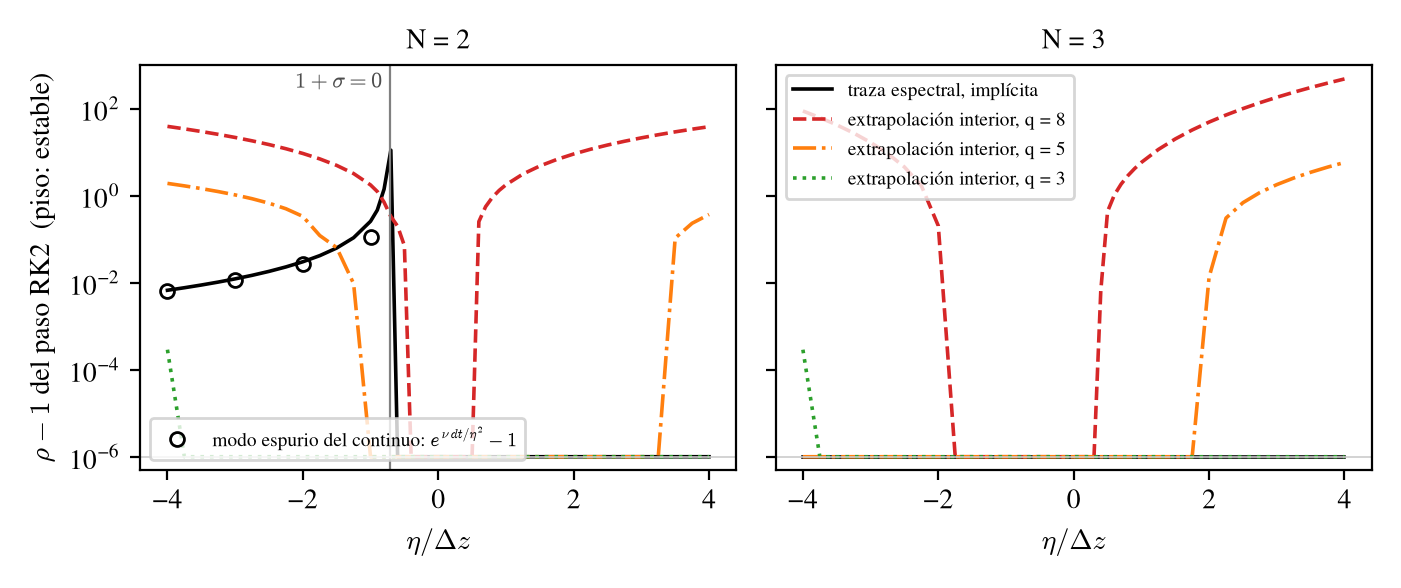
\includegraphics[width=0.93\textwidth]{f_fs6_estabilidad.png}
\vspace{-6pt}
\caption{\small Réplica 1D del paso RK2 de SPECTER: difusión FC-Gram, \texttt{neumann\_reconstruct}
y el dato de orden $N$ con $\eta$ constante; $\nu=0{,}01$, $dt=10^{-3}$, $n_z=128$. El eje
vertical es el radio espectral del paso menos uno; el piso es estable. Los círculos son la tasa
del modo espurio del continuo, $e^{\nu\,dt/\eta^2}-1$. Sale de
\archivo{numerico/fase6/estabilidad_cierre.py}.}
\label{fig:estab}
\end{figure}

\paragraph{(i) El cierre congelado era inestable.} Antes de programar había decidido
extrapolar $\partial_z^{m\ge2}u$ desde nodos interiores, porque la traza espectral responde al
dato como $1{,}4/\Delta z$ y la iteración ingenua diverge para $\eta>0{,}7\Delta z$. Con
extrapolación la iteración converge, pero el paso en el tiempo explota: la primera corrida con
$\eta=4\Delta z$ dio NaN. La réplica (figura~\ref{fig:estab}, líneas cortadas) lo explica. Para
$|\eta|>0{,}5\Delta z$ el nodo de borde queda como una extrapolación explícita con pesos $\sim600$
sobre el interior.

Las trazas espectrales resueltas \emph{implícitamente}, línea negra, son estables para todo
$\eta>0$ y para todo $\eta$ a $N=3$. Me quedé con esas, y el precondicionador de §2 es lo que
permite resolverlas.

\paragraph{(ii) El orden 2 está mal planteado donde $\eta<0$\propio.} La condición transferida
$\partial_zu+\eta\,\partial_{zz}u=0$ admite $u\propto e^{\lambda t}e^{\kappa(z-L_z)}$ con
$\kappa(1+\eta\kappa)=0$. Si $\eta<0$, la raíz $\kappa=1/|\eta|$ decae hacia el interior y da
$\lambda=\nu/\eta^2>0$: una capa espuria de espesor $|\eta|$ que crece.
\begin{itemize}
\item Es el cero del polinomio de Taylor truncado de $e^{\kappa\eta}$, que no tiene ceros.
\item El verificador lo confirmó en el problema 2D linealizado completo: la raíz es exactamente
  $\lambda=\nu(1/\eta_0^2-k^2)$.
\item La réplica reproduce la tasa del continuo cuando la capa está resuelta: con
  $\eta=-4\Delta z$, $\rho=1{,}00668$ contra $e^{\nu dt/\eta^2}=1{,}00652$.
\item En la malla, el umbral depende de $D=\nu\,dt/\Delta z^2$: el paso se vuelve inestable
  donde $1+\sigma\approx0{,}7D$. Con el $dt$ de la puerta eso es $\eta=-0{,}667\Delta z$, y en
  el límite $dt\to0$, $-0{,}716\Delta z$.
\item En SPECTER, con la guardia apagada, $N=2$ con $\eta_0=-0{,}01$ da NaN antes de $t=0{,}3$.
\end{itemize}
La guardia corta en $1+\sigma\le0{,}05+D$: con el $dt$ de la puerta, en $\eta=-0{,}607\Delta z$,
antes del umbral. Mi primera versión cortaba en $0{,}05$ y dejaba una ventana inestable sin
aviso; la encontró el verificador.

A $N=3$ los modos espurios son neutros para $\eta$ uniforme. Con pendiente $s$, según el
verificador (no lo reproduje), pueden crecer débilmente, con
$\mathrm{Re}\,\lambda\approx\nu(2s^2/\eta^2-k^2)$. Su segunda ronda encontró también que a $N=3$ el
paso es inestable cerca de $\eta=-1{,}2\Delta z$ a partir de $0{,}97$--$0{,}99$ del límite
explícito, $D_{\max}=0{,}205$. Eso sí lo reproduje, y $N=3$ exige ahora $D\le0{,}19$. \textbf{No cambié el modelo congelado}: un
orden 2 bien planteado queda como pregunta abierta \etq{P-04}.

\paragraph{(iii) Con elevación uniforme, $N=2$ ya es $O(\eta^3)$\propio.} Para $\phi\propto\cosh kz$
se tiene
\[
\frac{s+c\varepsilon}{c+s\varepsilon}-\tanh(kh+\varepsilon)=
\frac{\varepsilon\cosh\varepsilon-\sinh\varepsilon}{(\ldots)}=\frac{\varepsilon^3/3+\ldots}{(\ldots)}.
\]
En la primera versión escribí $-\varepsilon^3/2$; el coeficiente correcto, $+1/3$, lo dio el
verificador. La escalera de profundidad de la puerta (H5) pedía orden 2 a $N=2$: el criterio
estaba mal \emph{a priori}. La figura~\ref{fig:esc} muestra que SPECTER sigue al truncamiento
esperado.

\begin{figure}[h]
\centering
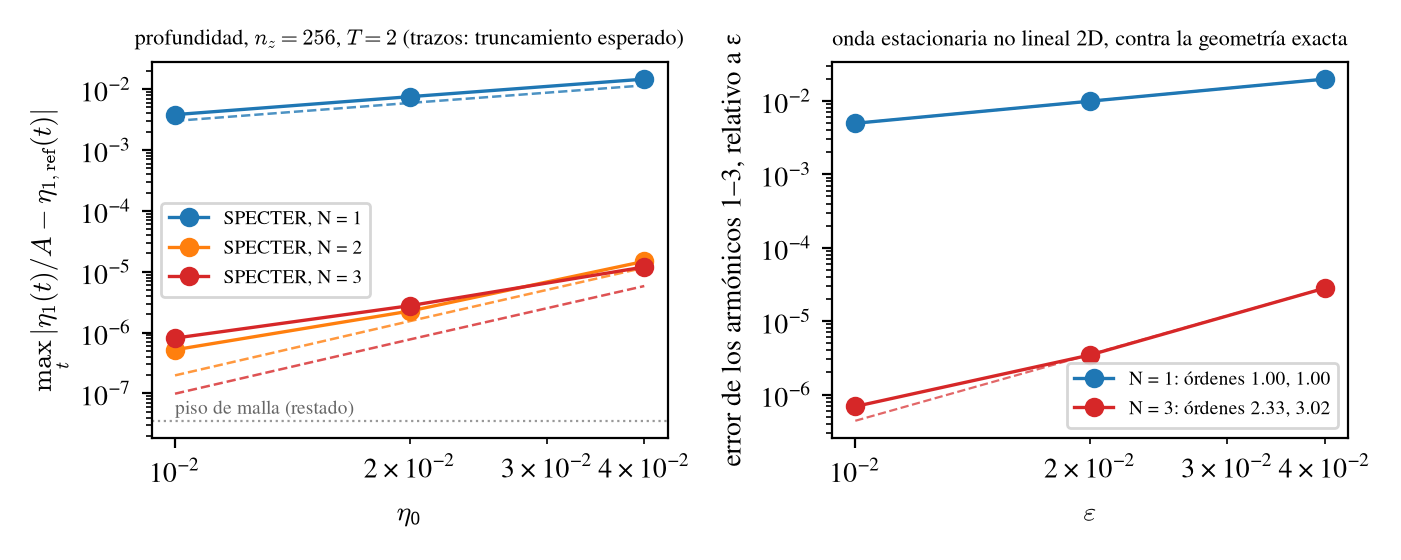
\includegraphics[width=0.97\textwidth]{f_fs6_escaleras.png}
\vspace{-6pt}
\caption{\small Izquierda: escalera de profundidad ($\eta_0$ uniforme, $n_z=256$,
$dt=2{,}5\cdot10^{-4}$, $T=2$). Los trazos son el truncamiento no viscoso esperado para cada $N$.
Derecha: la onda estacionaria no lineal 2D contra la geometría exacta, con la métrica de H7;
los trazos marcan las pendientes 1 y 3. Sale de \archivo{numerico/fase6/escaleras.py}.}
\label{fig:esc}
\end{figure}

\paragraph{(iv) $\partial_z^3u$ limita a $N=3$.} El error FC-Gram de la tercera derivada en el
borde \emph{no} baja como $\Delta z^2$, como creía. Tiene un mínimo cerca de $n_z=128$ y después
crece como $\Delta z^{-3}$: la continuación deja un piso determinista de
$\sim2\cdot10^{-11}|f|/\Delta z^3$. Para $\sin(1{,}2z)$ el error vale $1{,}8\cdot10^{-4}$,
$2{,}4\cdot10^{-4}$, $2{,}0\cdot10^{-3}$ y $1{,}7\cdot10^{-2}$ a $n_z=128$, 256, 512 y 1024. Lo
encontró el verificador y lo reproduje.

Con estas tablas, entonces, \textbf{$N=3$ no mejora refinando en $z$}. En la profundidad, con
$\eta_0=0{,}04$, $N=3$ pasa de $4{,}1\cdot10^{-5}$ ($n_z=128$) a $1{,}2\cdot10^{-5}$ ($n_z=256$);
ese $\times3{,}4$ no lo explica la traza, y el origen de ese exceso no está establecido. Donde no
hay degeneración, en la onda no lineal, $N=3$ tiene el orden esperado: \NLtresErr.

Además, la iteración tiene un piso de redondeo de algunos $10^{-9}$ con $\eta=4\Delta z$, que
nace en la traza $m=3$. Que escale como $\eta^2$ lo infiero del factor $\eta^2/2$; no lo medí.
Mi estimación de su tamaño omitía un $1/n_z$ (lo señaló el verificador), y su origen cuantitativo
queda abierto. Por eso el criterio de parada por estancamiento.

%=====================================================================
\section{La revisión independiente}

Un agente separado, con el rol «verifier» del equipo, reprodujo cada afirmación con su propio
código, sólo Python liviano (\archivo{numerico/fase6/verificador/}).
\begin{itemize}
\item \textbf{Verificó} el modelo, la fidelidad de la réplica al Fortran, $\beta_m$, la
  degeneración de la profundidad con viscosidad, el precondicionador, Anderson real y la
  convención de Nyquist. Su lectura adversarial del código encontró B1 y B4.
\item \textbf{Primera ronda: seis cosas.} Cinco las corregí:
  \begin{itemize}
  \item la ventana de la guardia;
  \item el coeficiente $+\varepsilon^3/3$;
  \item la cabecera de \texttt{fsorder.f90}, sin el término de $W$;
  \item que agotar \texttt{fsmaxit} era silencioso: ahora avisa;
  \item el $1/n_z$ de la estimación del piso.
  \end{itemize}
\item La sexta queda abierta: la inestabilidad débil de $N=3$ con pendiente, sin reproducir.
\item \textbf{Segunda ronda, sobre las correcciones:} confirmó la guardia nueva y encontró tres
  cosas más, que reproduje y corregí:
  \begin{itemize}
  \item $N=3$ cerca del límite explícito;
  \item el error de $\partial_z^3u$ que crece con $n_z$;
  \item afirmaciones viejas que quedaban en los documentos.
  \end{itemize}
\end{itemize}

%=====================================================================
\section{La puerta congelada: 4/10}

\begin{center}\small
\begin{tabular}{@{}llp{11.2cm}@{}}
\toprule
& & por qué\\
\midrule
H1 & \textbf{pasa} & el parser acepta 2 y rechaza 0 y 4\\
H2 & falla & trazas: $m=1$ da $3{,}5\cdot10^{-9}$ (umbral $10^{-9}$) y $m=3$ da $2{,}9\cdot10^{-4}$
(umbral $10^{-4}$). Los umbrales los fijé para el cierre descartado; son el piso FC-Gram\\
H3 & \textbf{pasa} & órdenes 1, 2, 3 (y 2, 2, 4 para $\kappa$) contra la geometría exacta\\
H4 & \textbf{pasa} & Fase 5 contra MAC $1{,}4\cdot10^{-6}$; camino general $N=1$ contra Fase 5 $2{,}5\cdot10^{-15}$\\
H5 & falla & criterio mal a priori (iii), más el piso de malla a $n_z=128$\\
H6 & \textbf{pasa} & la referencia se verifica: $6{,}6\cdot10^{-9}$, balance $2{,}8\cdot10^{-7}$\\
H7 & falla & aborta en su primer caso $N=2$ ($\eta$ llega a $-\Delta z$): (ii). Fuera de la
puerta, figura~\ref{fig:esc}: $N=1$ orden \NLunoOrd, $N=3$ orden \NLtresOrd\\
H8 & falla & es $N=2$ con $\eta$ hasta $-2\Delta z$: (ii)\\
H9 & falla & sólo por el residuo: $1{,}8\cdot10^{-9}$ contra $10^{-9}$, el piso (iv). Pasadas $\le12$ (tope 30), deriva de la media $10^{-16}$\\
H10 & falla & necesita la corrida $N=2$ de H7: (ii)\\
\bottomrule
\end{tabular}
\end{center}
La puerta está fijada por hash y no la edité; tampoco el intent. Lo que cambió respecto del
intent (el cierre de trazas y el criterio de parada) está registrado como decisión, con su
motivo.

%=====================================================================
\section{Qué sigue}
\begin{itemize}
\item Para la física, lo que importa es $N=2$ con $\eta/\Delta z\sim10^{-3}$, fuera de todo
  límite de arriba. El paso natural es correr el puente de banda ancha de \etq{V-19} con
  \texttt{fsorder = 2} y $g$, $\gamma$ físicos contra \texttt{freeslip}, para medir el efecto
  $O(\mathrm{Fr}^2)$ sobre $\alpha$. Con varias pasadas por subpaso es trabajo de Sakura.
\item \etq{P-04}: si hace falta $N=2$ con $|\eta|\gtrsim\Delta z$, una opción es llevar sólo la
  transferencia tangencial a orden 3. Así $1+\sigma$ ya no se anula, aunque hereda la
  inestabilidad débil con pendiente. Cambia el modelo congelado, así que lo decidís vos.
\item Una $\partial_z^3u$ de borde más precisa, por ejemplo desde la ecuación de momento en la
  frontera, haría que $N=3$ valga la pena a $n_z=128$.
\end{itemize}

\end{document}
